Com o objetivo de comparar o desempenho da implementação de co-rotinas com a biblioteca \textit{TOSThread}, foram
desenvolvidas duas aplicações para implementar o problema do produtor-consumidor.
Uma utilizando \textit{threads} (anexo~\ref{a:appTesteThread}), e outra utilizando co-rotinas (anexo~\ref{a:appTesteCoro}).
Foram utilizados uma linha de execução para o produtor, e outra para o consumidor, e um \textit{buffer} de tamanho
único. Para simular o tempo de processamento da produção e do consumo de uma unidade, foi implementado um laço de cem iterações, onde
cada passo executa uma operação aritmética. Após consumir mil produtos, uma nova linha de execução é ativada, para
calcular o tempo de execução.
%\begin{figure}
%\centering
%\includegraphics[scale=0.4]{images/ProdutorConsumidorTinyOS.png}
%\caption{Maquina de estados - Produtor/Consumidor}
%\end{figure}

O tempo de execução foi medido em uma plataforma \textit{MicaZ}, utilizando o temporizador
\textit{Counter<TMicro,uint32\_t>}, utilizando uma precisão de microsegundos. 
Os valores medidos não variaram mais de uma unidade entre as diferentes execuções e cada cenário foi executado dez
vezes.

No primeiro experimento, variamos a quantidade de produto, referente ao laço: 
\begin{lstlisting}
for (num_prods = 0 ; num_prods < 1000; num_prods++)
\end{lstlisting}
No segundo experimentos, variamos a quantidade de operações realizadas para simular a produção e o consumo, referente ao
laço:
\begin{lstlisting}
for (j = 0 ; j < 100; j++)
    counter *= 3;
\end{lstlisting}

Na figura \ref{grafico-experimentos-corotinas} podemos ver um gráfico com os resultados.
\begin{figure}
\centering
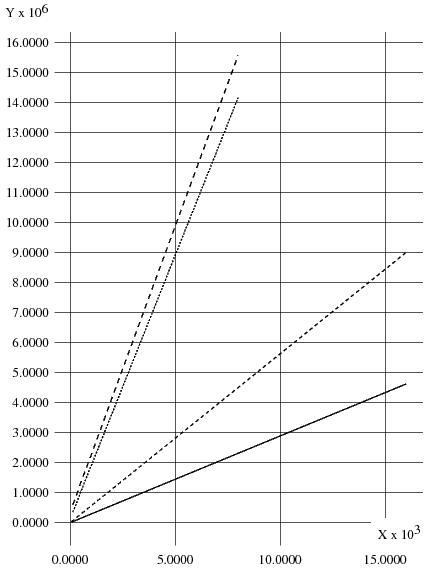
\includegraphics[scale=0.7]{images/grafico_coroXthreads2.png}
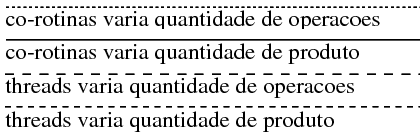
\includegraphics[scale=0.7]{images/legenda.png}
\caption{Gráfico dos experimentos de threads e co-rotinas}
\label{grafico-experimentos-corotinas}
\end{figure}


%Para variar a carga, foram utilizadas diferentes operações aritiméticas.
%O tempo de execução foi medido em uma plataforma \textit{MicaZ}, utilizando o temporizador
%\textit{Counter<TMicro,uint32\_t>}, utilizando uma precisão de microsegundos.
%Os valores medidos não variaram mais de uma unidade entre diferentes execuções.
%\begin{center}
%    \begin{tabular}{ | l | l | l | l | l | p{5cm} |}
%    \hline
%    Operação    & x += 1 & x *= 2 & x *= 3 & x *= 5 \\ \hline
%    Threads     & 380000 & 490000 & 530000 & 563000 \\ \hline 
%    Co-rotinas  & 151000 & 252000 & 289000 & 314000 \\ \hline 
%    \end{tabular}
%\end{center}
